\section{S1 -- Zasady projektowania sieci komputerowych}

Podczas projektowania architektury komutowanej sieci LAN (switched LAN) używa się modelu hierarchicznego sieci. Sieci w modelu hierarchicznym dzieli się na odrębne warstwy. Każda z nich realizuje określone funkcje, które definiują rolę danej warstwy w ogólnym modelu sieci. Budowa sieci przyjmuje postać modułową, co zwiększa jej skalowalność i efektywność działania.

\begin{itemize}
	\setlength\itemsep{1pt}
	\item[] {W modelu hierarchicznym można wyróżnić trzy warstwy:}
	\item warstwa dostępu (access layer),
	\item warstwa dystrybucji (distribution layer),
	\item warstwa rdzenia (córę layer).
\end{itemize}

\begin{figure}[H]
	\centering
	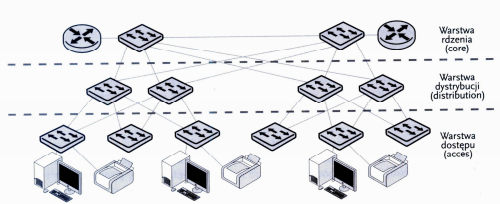
\includegraphics[width=\linewidth]{s1_hierarchiczny_model.png}
	\caption{Model hierarchiczny budowy sieci przełączanej}
\end{figure}

\textbf{Warstwa dostępu} jest sprzężona z takimi urządzeniami końcowymi, jak komputery PC, drukarki, telefony IP, a jej celem jest zapewnienie dostępu do pozostałych składników sieci. Jej głównym zadaniem jest:

\begin{itemize}
	\setlength\itemsep{1pt}
	\item umożliwienie połączenia urządzeń z siecią,
	\item umożliwienie kontroli nad komunikowaniem się urządzeń w sieci.
\end{itemize}

W warstwie dostępu mogą występować przełączniki, mosty, koncentratory i bezprzewodowe punkty dostępowe.

\textbf{Warstwa dystrybucji} gromadzi dane otrzymywane z przełączników z warstwy dostępu przed ich transmisją do warstwy rdzenia. Warstwa ta kontroluje przepływ danych w sieci oraz wyznacza domeny rozgłoszeniowe. Może również realizować routing między wirtualnymi sieciami LAN (VLAN - Virtual LAN), jeżeli na poziomie warstwy dostępu utworzono takie sieci.

\textbf{Warstwę rdzenia} stanowią szybkie łącza szkieletowe. W warstwie tej gromadzi się ruch sieciowy ze wszystkich urządzeń warstwy dystrybucji, a zatem musi być ona w stanie szybko przekazywać duże ilości danych. Warstwa rdzenia może być połączona z zasobami inernetowymi.

Aby zapewnione zostały maksymalne korzyści przy minimalnym nakładzie pracy i środków, sieć komputerowa powinna posiadać następujące cechy:

\begin{itemize}
	\setlength\itemsep{1pt}
	\item skalowalność,
	\item nadmiarowość,
	\item wydajność,
	\item bezpieczeństwo,
	\item łatwość zarządzania i utrzymania.
\end{itemize}

\textbf{Skalowalność} możemy rozumieć jako podatność sieci na rozbudowę. Rozrastanie się sieci o dużej skalowalności można łatwo zaplanować i realizować. Na przykład, przyjmijmy założenie, że na przełącznik z warstwy dystrybucji może przypadać dziesięć przełączników z warstwy dostępu. Wtedy dodatkowy przełącznik w warstwie dystrybucji trzeba będzie dodać do topologii sieci dopiero po przekroczeniu maksymalnej liczby dziesięciu podłączonych przełączników warstwy dostępu.

Zwiększenie niezawodności sieci można osiągnąć, wprowadzając \textbf{nadmiarowość} (redundancję) urządzeń lub/i ścieżek. W celu zapewnienia nadmiarowości poszczególne przełączniki z warstwy dostępu są łączone z więcej niż jednym przełącznikiem z warstwy dystrybucji (np. z dwoma różnymi przełącznikami z warstwy dystrybucji). Jeśli jeden z przełączników warstwy dystrybucji ulegnie awarii, to przełącznik z warstwy dostępu może współpracować z drugim przełącznikiem z tej warstwy. Z kolei przełączniki z warstwy dystrybucji są łączone z co najmniej dwoma przełącznikami z warstwy rdzenia. W warstwie dostępu nie występuje nadmiarowość - urządzenia końcowe (komputery, drukarki itp.) nie mogą być przyłączone do więcej niż jednego przełącznika. Jeśli w warstwie dostępu wystąpi awaria przełącznika, to będzie mieć wpływ tylko na urządzenia, które są do niego podłączone.

\textbf{Wydajność} komunikacji można poprawić, unikając transmisji danych przez niskowydajne przełączniki pośredniczące. W warstwie dystrybucji powinny być stosowane przełączniki o wydajności większej niż w warstwie dostępu. Przełączniki w warstwie rdzenia powinny mieć najwyższą wydajność, aby zapewnić szybkie przesyłanie dużej ilości danych. Zastosowanie w warstwie dostępu tańszych przełączników i zwiększenie nakładów na przełączniki z warstw dystrybucji i rdzenia pozwala uzyskać jednocześnie wysoką wydajność sieci i oszczędności finansowe.

Profesjonalne przełączniki umożliwiają \textbf{zwiększenie bezpieczeństwa} poprzez wprowadzenie zasad ograniczających dostęp do sieci. Przełączniki z warstwy dostępu można kon-figurować, stosując różne opcje zabezpieczeń portów (port security) oraz sieci wirtualne VLAN, zapewniające kontrolę nad tym, które urządzenia mogą się łączyć z siecią.

W trakcie rozrastania się sieci jej utrzymanie staje się coraz bardziej skomplikowane. Urządzenia stosowane w danej warstwie powinny posiadać podobne parametry techniczne i konfigurację. Dla zapewnienia \textbf{łatwości zarządzania i utrzymania} można stosować jednakowe urządzenia. Jeśli trzeba będzie zmienić funkcjonalność jakiegoś przełącznika, np. z warstwy dostępu, to zmianę tę można powielić we wszystkich przełącznikach z tej warstwy, gdyż najprawdopodobniej wykonują one te same funkcje. Wdrażanie nowych przełączników jest ułatwione, ponieważ ich konfiguracje można skopiować z innych urządzeń i ewentualnie wprowadzić niewielkie modyfikacje.


\begin{enumerate}
	\item[] \textbf{Przykładowe Etapy projektowania sieci: }
	\item Inwentaryzacja,
	\item Poznanie i analiza potrzeb użytkownika,
	\item Wynikające z analizy założenia projektowe,
	\item Projekt sieci:
	\begin{enumerate}
		\item Projekt logiczny sieci,
		\item Projekt okablowania (poziome – użytkownik punkt dystrybucyjny, pionowe – pomiędzy punktami dystrybucyjnymi),
		\item Konfiguracja adresacji,
		\item Podłączenie do Internetu,
		\item Bezpieczeństwo i niezawodność sieci,
		\item Kosztorys
	\end{enumerate}
\end{enumerate}